\documentclass{standalone}

\usepackage{pgfplots}
\pgfplotsset{compat=1.9}
\usetikzlibrary{backgrounds}

\pgfplotsset{grid style={dotted, black}}

\begin{document}
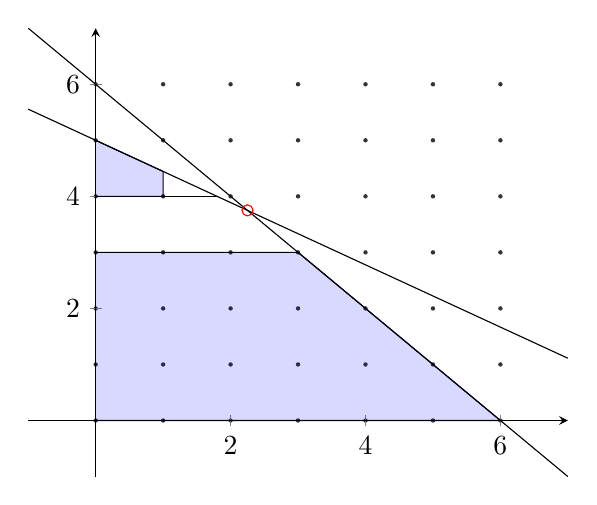
\begin{tikzpicture} 
  \begin{axis}[enlargelimits=0.1, axis lines=middle,after end axis/.code={%
    \begin{scope}[on background layer]
    \foreach \x in {0,...,6}{
    \foreach \y in {0,...,6}{
    \fill[black!80] (axis cs:\x,\y) circle[radius=0.8pt];
    }}\end{scope}
    }]
  \addplot[domain=-1:7,fill=gray!50] {6 - x};
  \addplot[domain=-1:7,fill=gray!50] {(45 - (5*x)) / 9};
  \addplot [color=transparent,fill=blue, 
            fill opacity=0.15]coordinates {
            (0,4)
            (1,4)
            (1,40/9)
            (0,5)};
  \addplot[]coordinates {(1,4) (9/5,4)};
  \addplot [color=transparent,fill=blue, 
            fill opacity=0.15]coordinates {
            (0,0)
            (6,0)
            (3,3)
            (0,3)};
    \draw[red] (axis cs:9/4,15/4) circle[radius=2pt];
    \end{axis}
\end{tikzpicture}  
\end{document}